\section{Resting atmosphere}
Compared meshes, and dp/dx versus H operator.

\begin{itemize}
\item Max vertical velocities compared in Figure~\ref{fig:rest:w}
\item Energy change compared (see Figure~\ref{fig:rest:energy-tf}, \ref{fig:rest:energy-cut-cell})
\item H operator always outperforms dp/dx
\item All cut-cell style meshes outperform TF meshes in this test in terms of $w$ and energy change
\end{itemize}
Some issues were found:
\begin{itemize}
\item noOrography should have zero $w$, but actually has \SI{1e-10}{\meter\per\second}.  Hilary says this is due to loss of precision when reading initial fields (should be in discrete hydrostatic balance).
\item Computational oscillation in BTF H operator after about 4 hours (Figure~\ref{fig:rest:energy-tf})
\end{itemize}

\begin{figure}
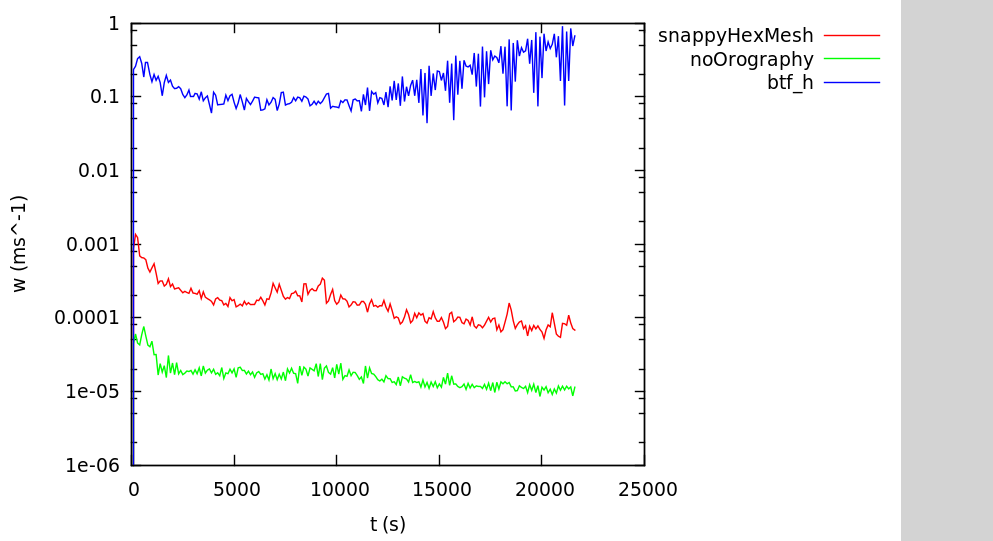
\includegraphics[width=\textwidth]{interim-results/verticalVelocityPlotSnappyHexMesh.png}
\caption{Max vertical velocities (note log scale on y axis)}
\label{fig:rest:w}
\end{figure}

\begin{figure}
BTF H
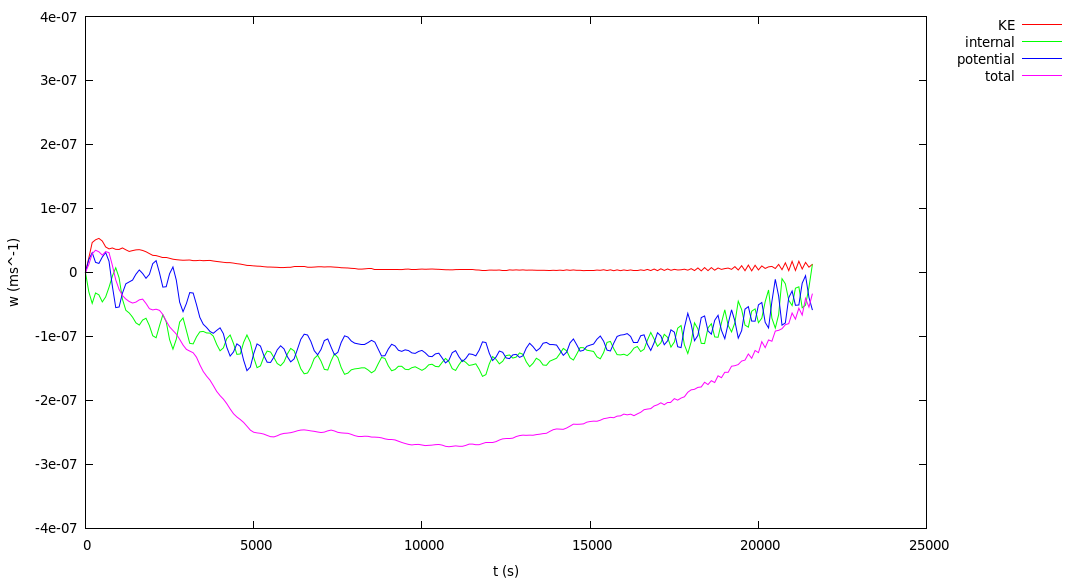
\includegraphics[width=\textwidth]{interim-results/restingBtfHEnergy.png}
SLEVE
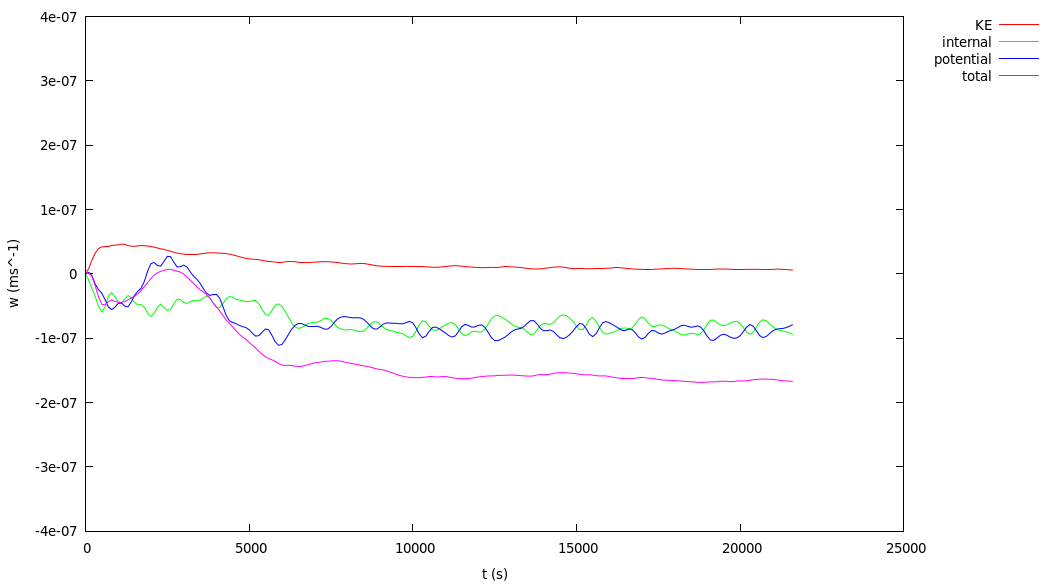
\includegraphics[width=\textwidth]{interim-results/restingSleveEnergy.png}
\caption{Energy changes (TF)}
\label{fig:rest:energy-tf}
\end{figure}

\begin{figure}
SnapCol
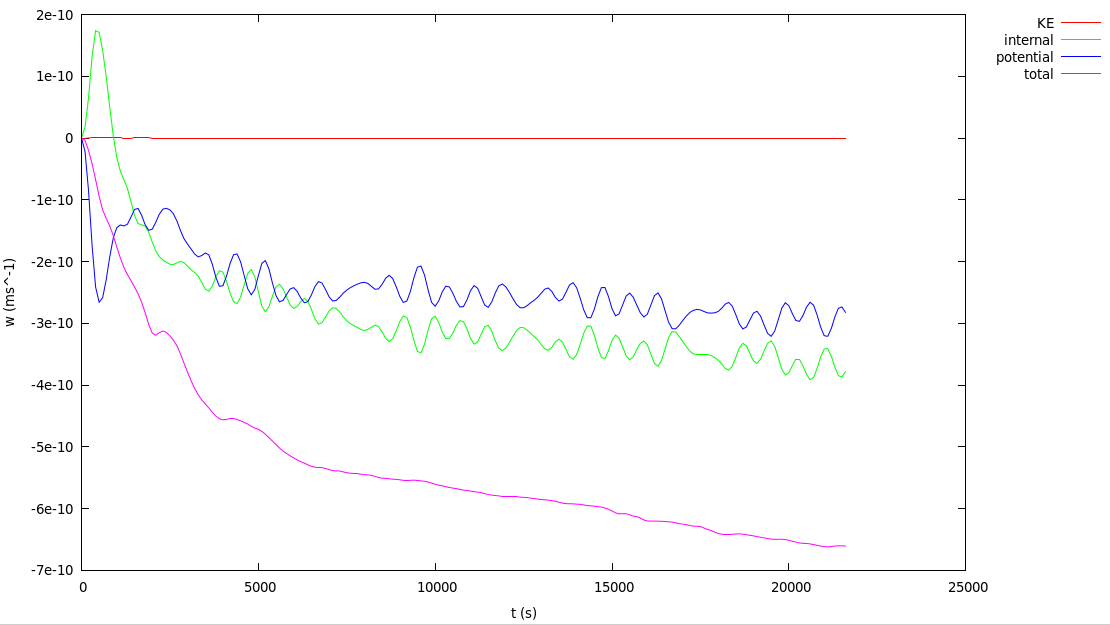
\includegraphics[width=\textwidth]{interim-results/restingSnapColEnergy.png}
Snap
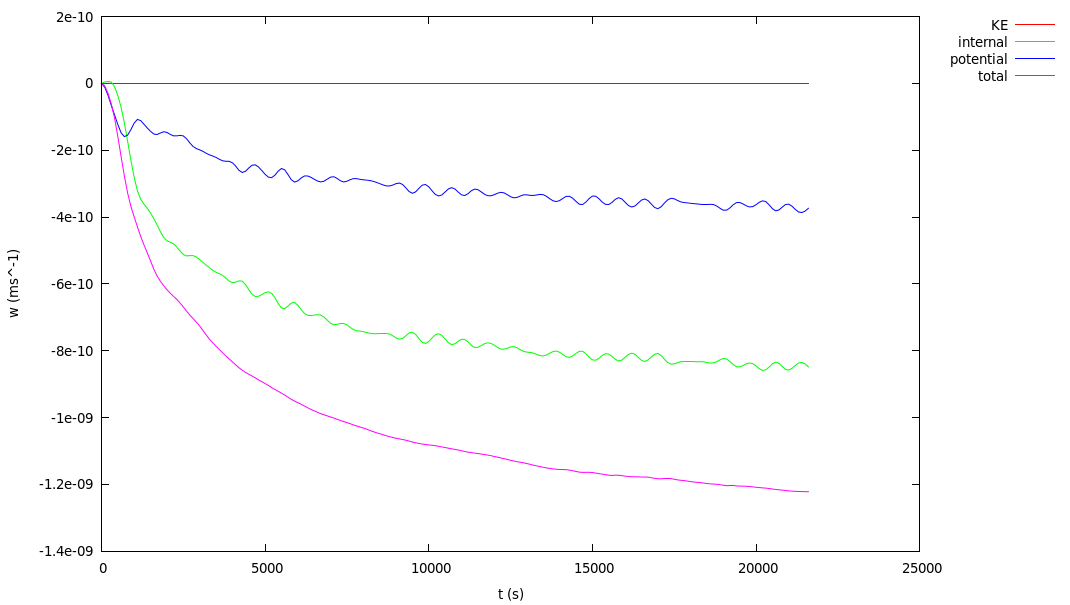
\includegraphics[width=\textwidth]{interim-results/restingSnapEnergy.png}
\caption{Energy changes (cut-cell style)}
\label{fig:rest:energy-cut-cell}
\end{figure}
